
% \newcommand{\Suffix}[2]{ {#1}^{\overset{#2}{\leftarrow} } }
% \newcommand{\Suffix}[2]{ {#1}[-{#2}:] }
\newcommand{\Suffix}[2]{ \mathsf{suffix}({#1},{#2})}
\newcommand{\CoinTossingLC}{\Pi_\mathsf{lc}^{\Players(\alpha),k,n}}

Let $\EpsP \in (0,1)$ and $s, k \in \NN$. 
Let $\Blockchain$ be an $(\EpsP, k, s)$-secure eventual consensus PoS blockchain protocol 
under the longest-chain rule, such as 
Ouroboros Praos~\cite{Praos} and Snow White~\cite{SnowWhite}.

Let $\kappa, n \in \NN$.
When the protocol $\Blockchain$ commences, 
all participants in $\Blockchain$ are given a 
(publicly known) uniformly random string $\eta_0 \in \{0,1\}^\kappa$. 
$\Blockchain$ utilizes an $n$-slot 
coin-flipping sub-protocol $\Pi = \CoinTossingLC$ 
which takes $\eta_0$ as input 
and produces an output $\eta_{t} \in \{0,1\}^\kappa$. 
The coin-flipping protocol $\Pi$ has a simple description, as follows:
\begin{enumerate}
  \item For slots $i \in [n]$, 
  every new block added during slot $i$ contains a uniformly random string; 
  it is called a \emph{nonce}.

  \item At the end of slot $n + k$, 
  anyone can compute the output $\eta$
  as the exclusive-OR of all nonces recorded in his locally-held blockchain. 
\end{enumerate}
% The goal of this section is to derive positive reals $\EpsP \in (0, 1)$ and $\rho \in (0, \kappa)$ 
% so that the protocol $\Pi$ is $(\EpsP, \rho)$-secure. 
% Specifically, we have the following: 

\begin{theorem}\label{thm:minentropy-loss-praos}
  Let $\alpha \in (0, 1/2)$ and $\tau, n, k, s \in \NN$. 
  % so that $\alpha^n \leq 2^{-\tau}$.
  % Let $W$ be a characteristic string of length $n$ so that 
  % the symbols in $W$ are i.i.d. 
  % with $\Pr[W_t = \A] = \alpha$ for $t \in [n]$.
  Suppose the adversarial players control at most an $\alpha$ fraction of relative stake 
  in $\Blockchain$ 
  which runs for $n$ slots where 
  each slot is independently assigned to some adversarial player 
  with probability $\alpha$. 
  Let $E$ denote the event that 
  $\Blockchain$ 
  remains $(2^{-\tau}, k, s)$-secure throughout this execution. 
  Then $\Pi$ is $(2^{-\tau + 1}, \rho)$-secure, where 
  \begin{align}
      % \qquad\text{and}\qquad
      % \beta &= \\
    \rho &= \log_2 n + \tau/2 + n \cdot 
      \begin{cases}
        % 0.43 (1 - 2\alpha)
        %     \,, &\quad\text{if}\quad\epsilon \in (0, 1/3]\,, \\
        % 0.24 (1 - 2\alpha) (5/2 - 3 \alpha)
        % % 15/16 - 0.24 \epsilon(1+\epsilon)(1-\epsilon/2)
        %     \,, &\quad\text{if}\quad\epsilon \in (1/3,0.809]\,, \\
        % 2/3
        %     \,,&\quad\text{otherwise}\,.
        0
            \,, &\quad\text{if}\quad\alpha \in (0, 0.0955)\,, \\
        0.067 + 1.92 \alpha - 1.44 \alpha^2
            \,, &\quad\text{if}\quad\alpha \in [0.0955, 1/3)\,, \\
        0.237 + 0.86 \alpha
            \,, &\quad\text{if}\quad\alpha \in [1/3, 1/2)\,.
      \end{cases}    
    % \,.
  \end{align}
\end{theorem}
The theorem above is a straightforward corollary 
of Theorem~\ref{thm:praos-tail-gamma} 
(using $\alpha = (1 - \epsilon)/2$ 
and $\EpsG = 2^{-\tau}$ in that theorem).
Observe that for $\alpha \geq 0.0955$, 
the min-entropy loss depends linearly on $n$ 
which is typically $\Omega(k)$. 
In contrast, in Section~\ref{sec:coin-tossing}, 
we develop coin-flipping protocols (with an integer parameter $d$) 
where we can effectively ``slow down'' the growth of $\rho$ by a factor $1/d$.
Specifically, 
in those protocols, nonces are associated with slots.
the minentropy-loss in those protocols 
depends linearly on $k/d$ 
but logarithmically on $n/d$; 
hence we can avoid a loss in $\rho$ 
by suitably increasing the failure probability.
It is not obvious how to do the same for protocol $\Pi$, however, 
as nonces are associated with blocks, not slots. 


\iftoggle{drawfigs}{

\begin{figure}
  \centering
  \pgfmathsetmacro{\k}{100}
  \pgfmathsetmacro{\d}{1}
  \pgfmathsetmacro{\T}{24 * \k}
  \pgfmathsetmacro{\tau}{30}
  \pgfmathsetmacro{\n}{(\T - \k)/\d}
  \pgfmathsetmacro{\ell}{\k/\d}
  \pgfmathsetmacro{\ellPlusN}{\ell + \n}
  \begin{tikzpicture}[trim axis left,
    declare function={rho_praos_small_alpha(\a) = log2(\n + \ell) + \tau / 2 ; 
      rho_praos_mid_alpha(\a) = log2(\n + \ell) + \tau / 2 + \n * (0.067 + 1.92*\a - 1.44 * \a * \a) ; 
      rho_praos_large_alpha(\a) = log2(\n + \ell) + \tau / 2 + \n * (0.237 + 0.86 * \a); 
      rho_geom_small_alpha(\a) = 2 * log2(\n) + \tau/2 + \ell * log2( sqrt(1 + \a)/(1 - \a) );
      rho_geom_large_alpha(\a) = 2 * log2(\n) + (\tau + \ell * log2( 1/\a ) )/(2 - (3 * \a - 1)/(2 * \a * \a));
    }
    %    declare function = { entropy(\x) = 1; },
    ]
    \begin{axis}[domain=0:0.5,
      samples=100,
      enlarge x limits=false,
      grid=both,
      no markers,
      x label style={at={(axis description cs:0.5,-0.1)},anchor=north},
      y label style={at={(axis description cs:-0.1,.5)},anchor=south},
      xlabel={$\alpha$, relative adversarial stake},
      ylabel={$\rho$, loss in min-entropy (bits)},
      % there is one default value for the `legend pos' that is outside the axis
      legend pos=outer north east,
      % (so the legend looks a bit better)
      legend cell align=left
      ]
      \addplot +[thick,domain=0:(0.0955),red,forget plot] plot (\x, {rho_praos_small_alpha(\x)});
      \addplot +[thick,domain=0.0955:(1/3),red,forget plot] plot (\x, {rho_praos_mid_alpha(\x)});
      \addplot +[thick,domain=(1/3):(0.5),red,legend] plot (\x, {rho_praos_large_alpha(\x)});
      \addlegendentry{Praos, $\ellPlusN$ rounds}

      \addplot +[thick,domain=0:(1/3),blue,forget plot] plot (\x, {rho_geom_small_alpha(\x)});
      \addplot +[thick,domain=(1/3):(1/2),blue,legend] plot (\x, {rho_geom_large_alpha(\x)});
      \addlegendentry{$(\ell, \n, \alpha)$-geometric game, $d = 1$}
    \end{axis}
  \end{tikzpicture}
  \caption{Min-entropy loss in Praos (red) and in the $(\ell, n, \alpha)$-geometric game (blue).}
  \label{fig:rho-praos}
\end{figure}

} % end iftoggle{drawfigs}


As we discussed after Definition~\ref{def:coin-flipping-security}, 
the adversarial participants in an $(\EpsP, \rho)$-secure 
coin-flipping protocol $\Pi$ can choose the output $\eta$ 
from a set $X$ of size $2^\rho$. 
As $\Pi$ is conducted on the blockchain protocol $\Blockchain$, 
the elements of $X$ are determined by 
the set $C$ of all possible maximally long blockchains 
at (or after) slot $n + k$. 
Due the the $\kSlotCP$ property of $\Blockchain$, 
these chains contain the same blocks corresponding to slots $1, \ldots, n$. 
It follows that $\rho = \log_2 |X| = \log_2 g$.
% We call $g$ the \emph{grinding power} of the adversary. 

\subsection{Viable blockchains and grinding power}

The leader election process of $\Blockchain$ associates, 
with each round $t = 1, 2, \ldots$, 
a set of participants (called \emph{leaders}) 
that are entitled to add a block at round $t$ to a blockchain. 
We can represent the outcome of this leader election scheme 
as a \emph{characteristic string}.


\begin{definition}[Characteristic string]\label{def:bivalent-char-string}
  Let $n \in \NN$.
  A \emph{characteristic string} $w$ 
  is an element of $n$ symbols where 
  each symbol is either $\A$ or a positive integer. 
  It is defined for a particular execution of a blockchain protocol 
  on slots $1, \ldots, n$ so that 
  for each slot $t \in [n]$, 
  $w_t = \A$ if $t$ is assigned to an adversarial participant; and 
  $w_t = k$ if $t$ is assigned to $k$ honest participants, $k \geq 1$, 
  but no adversarial participants.
  By convention, set $w_0 = 1$.
\end{definition}

% \begin{definition}[Characteristic string]\label{def:trivalent-char-string}
%   Let $\slot_1, \ldots, \slot_{n}$ be a sequence of slots. 
%   A \emph{characteristic string} $w$ 
%   is an element of $\{\h,\H,\A\}^n$ 
%   defined for a particular execution of a blockchain protocol on these slots so that 
%   for $t \in [n]$, 
%   $w_t = \A$ if $\slot_t$ is assigned to an adversarial participant; otherwise, 
%   $w_t = \h$ if $\slot_{t}$ is assigned to a single honest participant; 
%   otherwise, $w_t = \H$.
% \end{definition}
For two strings $x$ and $w$ on the same alphabet, 
we write $x \Prefix w$ iff $x$ is a strict prefix of $w$. 
Similarly, 
we write $x \PrefixEq w$ iff either $x = w$ or $x \Prefix w$. 
The empty string $\varepsilon$ is a prefix to any string. 
If $w_t = \A$, we say that ``$\Slot_t$ is adversarial'' and 
otherwise, we say that ``$\Slot_t$ is honest.'' 
Define $\#_\A(w)$ as the number of occurrences of $\A$ in $w$. 
Define $\#_\h(w) \triangleq |w| - \#_\A(w)$.
An slot $t$ is called \emph{$k$-honest} if 
$t$ is an honest slot in $w$ and $w_t = k$.
A characteristic string $w$ is called $\Hheavy$ if 
$\#_\h(w) > \#_\A(w)$; 
otherwise, $w$ is called $\Aheavy$. 
We use $w[i : j]$ to denote the substring $w_i w_{i+1}\ldots w_j$ 


Consider an abstract execution of $\Blockchain$ 
corresponding to the characteristic string $w$ 
where 
all blockchains are arranged in a rooted tree; 
this tree is called a \emph{fork}. 
Two blockchains $\Chain_1, \Chain_2$ in a fork $F$ are considered ``different'' 
if and only if there is a slot from which 
$\Chain_1$ contains a block but $\Chain_2$ does not. 
A blockchain $\Chain \in F$ is \emph{viable} or \emph{competitive} 
if $\vert \Chain \vert$ is at least $\#_\h(w)$. 
The rationale is that an honest blockchain $\Chain$ is broadcast immediately 
and hence all blockchains adopted in the future 
must be at least as longa as $\Chain$. 
In addition, if an honest participant is presented with 
a blockchain $\Chain$ with length at least $\#_\h(w)$, 
that participant would possibly prefer $\Chain$ 
over a blockchain containing only honestly-emitted blocks 
as we assume that any tie is broken by the adversary. 

Considering any fork $F$ and an honest blockchain $\Chain$ in $F$, 
a \emph{viable adversarial extension of $\Chain$} 
is another blockchain $\Chain' \in F$ 
such that $\Chain$ is a prefix of $\Chain'$, 
$\Chain'$ is a maximally long blockchain in $F$, 
and, importantly, $\Chain'$ contains only adversarial blocks after the prefix $\Chain$. 
Note that every adversarial extension yields a choice 
for the coin-flipping output $\eta$.
Thus we focus on upper bounding, 
for any execution on $w$, 
the total number of viable adversarial extensions 
of the honest blocks.
Note that a prerequisite to creating an adversarial extension 
an honest slot $h$ is that 
the suffix $w[h + 1 : n]$ must be $\Aheavy$.
We formalize this notion in the definition below.

\begin{definition}[Option Sequences and Grinding Power]\label{def:option-sequence}
  Let $w$ be a characteristic string of length $n$. 
  We say that a sequence
  \[
    0 \leq i_0 < i_1 < \cdots < i_k \leq n
  \]
  is an \emph{option sequence} if
  \InlineCases{
    \item $i_0 = 0$ or 
    % $w_{i_0} = \h$, 
    $i_0 \neq \A$, 
    \item $w_{i_j} = \A$ for each $j > 0$, and
    \item $k \geq \#_\h(w[i_0 +1 : n])$.
  }
  We define the \emph{grinding power} of $w$, denoted $g(w)$, to be the
  number of distinct option sequences for $w$.
\end{definition}

% Let $\Suffix{w}{d}$ denote the length-$d$ suffix of a string $w$.

% Fix a characteristic string $w$ of length $n$.
%  and 
% let $x = \Suffix{w}{d}$. 
% Condition on the event that $\#_\h(x) = z$.
% The grinding power of $x$, which we denote by $g\left( x \Given \wt(x) = d - z  \right)$, 
% equals the number of distinct option sequences corresponding to $x$ 
% defined as
For any characteristic string $y$, define 
\begin{equation}\label{eq:S_y}
    % S(d, z) 
    % \defeq \sum_{i \geq z}^{d - z}{ \binom{d - z}{i} } 
    S(y) 
    \defeq \sum_{i \geq \#_\h(y)}^{\#_\A(y)}{ \binom{\#_\A(y)}{i} } 
    \,.
\end{equation}
Let $w = xy$ be a characteristing string. 
Then $S(y)$ is the number of viable blockchains $\Chain$
in an execution on $w$ 
so that the last honest block in $\Chain$ occurs in slot $|x|$. 
Thus the total number of viable blockchains for $w$ is 
\begin{equation}\label{eq:g_praos}
    g(w) 
    % = \sum_{d=1}^n g(\Suffix{w}{d})
    = \sum_{\substack{x,y : w = xy, \\ |x| \geq 0, \\ \text{and $|x|$ is honest} }} w_{|x|}\, S(y)
    \,.  
\end{equation}

\subsection{A tail bound on the grinding power}
Let $\epsilon \in (0, 1), \alpha = (1 - \epsilon)/2$, and 
let $W = W_1 \ldots W_n$ be a characteristic string of length $n$ so that 
the symbols in $W$ are independent and identically distributed 
with $\Pr[W_t = \A] = \alpha = (1 - \epsilon)/2$ for $t \in [n]$.
Think of $\epsilon$ as the ``adversarial bias.'' 
Define 
\begin{align}\label{eq:suffix-prob-binomial}
    B_{n, \epsilon}(k) 
    &= \Pr[ \#_\A(W_1 \ldots W_n) = k ]  
    = 2^{-n}\binom{n}{k} (1-\epsilon)^k (1 + \epsilon)^{n-k} 
    =  \binom{n}{k} 
        \left(\frac{1-\epsilon}{2}\right)^n 
        \left(\frac{1 + \epsilon}{1-\epsilon} \right)^{n-k} 
        \,.
\end{align}
Define
\begin{equation}\label{eq:prob-Hheavy}
  h(n) 
  \triangleq \Pr[\text{$W$ is $\Hheavy \mid W$ has length $n$}] 
  = \sum_{k \geq n/2} B_{n, \epsilon}(k)
  \,.
\end{equation}
Define
\begin{equation}\label{eq:S_d_z}
  S(d, z) = S(y) \quad\text{where $y$ is a characteristic string with $|y| = d$ and $\#_\h(y) = z$}
  \,.  
\end{equation}
Let $\lambda$ be a positive real, $\lambda \geq 1$. 
% (For our application, we would only use $\lamba = 2$.)
We can express the $\lambda$-th moment of the grinding power as
\begin{align}\label{eq:grinding-power-moment-praos}
    \Exp\, g(W)^\lambda 
    &\leq \sum_{\substack{x,y : W = xy, |x| \geq 0, \\ \text{and $|x|$ is honest} }} 
      \Exp\, g(y)^\lambda \nonumber \\
    &= \sum_{\substack{x,y : W = xy, |x| \geq 0, \\ \text{and $|x|$ is honest} }}\, \sum_{k \geq 1} 
      \Pr[\text{$W_{|x|} = k$ and $y$ is $\Aheavy$}] \cdot k^\lambda\, S(y)^\lambda \nonumber \\
    &=  %\Pr[\text{$W_1$ is honest}]\,
        \underbrace{\sum_{k\geq 1} \Pr[W_1 = k]\, k^\lambda}_{A(\epsilon, \lambda)} 
        \cdot 
        \sum_{d=1}^n \sum_{z = 0}^{ d/2 } B_{d, \epsilon}(d - z) S(d,z)^\lambda
\end{align}
with the convention that 
the inner sum runs for $z = 0, 1, \ldots, \lfloor d/2 \rfloor$. 
Here, the first inequality follows from 
the subadditivity of the convex function 
$x \mapsto x^\lambda$ for $\lambda \geq 1, x \geq 0$,  
and~\eqref{eq:g_praos}. 
The last equality follows from the independence of the symbols in $W$ 
and~\eqref{eq:S_d_z}.
Our goal is to develop a tight upper bound on $\Exp g(W)^2$ 
which, when used in Markov's inequality, 
would give us a tail bound on $g(W)$. 
{\color{blue}It turns out that the the second moment of $g(W)$ grows 
much faster than its first moment. In fact, 
Chebyshev's inequality on $g(W)$ fares only marginally better 
than what we get via Markov's inequality on $g(W)^2$. 
Thus we defer the analysis of the first moment in Appendix~\ref{app:grinding-praos}.}


\begin{claim}\label{claim:multiple-honest-blocks}
  For $\epsilon \in (0, 1)$, 
  $$
    A(\epsilon, 2) 
    \leq 
    \frac{(1 + \epsilon)^2 (5 + \epsilon)}{16 \left( 1 - e^{(1 + \epsilon)/2} \right)}
    \leq 2^{- 0.3 + 1.85 \epsilon}
    \,.
  $$
\end{claim}



% $\Exp H_m^2 \leq \Exp \GeomOneMinusAlpha^2 = (2 - \alpha)/\alpha^2$. 
% The last equality is a known fact; see~\eqref{eq:geom-moments-1-2} 
% which gives the second moment of $\GeomAlpha$. 
% Therefore,
% \begin{align}
%   \sum_{k\geq 1} \Pr[W_1 = k]\, k^\lambda 
%   &\leq \frac{1 - \alpha}{1 - e^{-(1 - \alpha)}} \frac{2 - \alpha}{\alpha^2} \nonumber \\
%   % &= \frac{1+\epsilon}{2} \frac{3 + \epsilon}{2} \frac{4}{(1 - \epsilon)^2}
%   &= \frac{(1+\epsilon)(3 + \epsilon)}{(1 - \epsilon)^2\left( 1 - e^{-(1 + \epsilon)/2} \right)}
%   \,.
% \end{align}



\begin{claim}\label{claim:t1star-variance-exact}
  Let $\epsilon \in (0,1)$ and 
  let $d,z$ be non-negative integers where $d \geq 2$ and $z \leq d/3$. 
  \begin{align*}
    B_{d, \epsilon}(d-z) S(d,z)^2
    &\leq \begin{dcases} 
    \left( (5-3 \epsilon)/2 \right)^d \,,
        &\quad \text{if}\quad
        0 < \epsilon < 1/3 \,, \\
    \left( 2^{2/3} \phi(\epsilon) \right)^d \,,
    %\frac{6}{\sqrt{5 d}}
        &\quad \text{if}\quad
        1/3 \leq \epsilon < 1 \, ,
    \end{dcases}
  \end{align*}
  where
  \begin{align}
    \phi(\epsilon) 
    &\triangleq \frac{3}{2} (1+\epsilon)^{1/3} (1-\epsilon)^{2/3}\label{eq:phi_eps} 
    \,.
  \end{align}
\end{claim}

\begin{claim}\label{claim:t2star-variance-exact}
  Let $\epsilon \in (0,1)$ and 
  let $d,z$ be non-negative integers where $d/3 \leq z \leq d/2$. 
  \begin{align*}
    B_{d, \epsilon}(d-z) S(d,z)^2
    &\leq \begin{cases} 
    \left( 2^{2/3} \phi(\epsilon) \right)^d \,,
        &\quad\text{if}\quad 0 < \epsilon \leq 0.6\,, \\
    \left( (5/3) \phi(\epsilon)  \right)^d \,,
        &\quad\text{if}\quad 0.6\leq \epsilon < 0.81\,, \\
    1 \,,
        &\quad\text{if}\quad 0.81 \leq \epsilon < 1
        \,.
    \end{cases}
  \end{align*}
\end{claim}
We defer the proofs of these claims in the next subsection .


% \subsection{Moment-bounds on the grinding power}

% \begin{lemma}[First moment of the grinding power]\label{lemma:grinding-power-mean}
% Let $W \sim \Binomial(n, (1-\epsilon)/2)$ for $\epsilon \in (0,1)$. 
% Then
% \begin{align*}
%     \phi(\epsilon)^n/4 \leq \Exp g(W) \leq n\, \gamma(\epsilon)^n
%     \,,\qquad\text{if}\quad \epsilon < 0.6\,, \\
%     \ln(n)/2 \leq \Exp g(W) \leq n
%     \,,\qquad\text{if}\quad \epsilon \geq 0.6\,,
% \end{align*}
% where
% \begin{align}
%     \gamma(\epsilon) 
%     &\defeq (1-\epsilon)/2 + \sqrt{1-\epsilon^2} \label{eq:gamma_eps}
%     \,.
% \end{align}

% \end{lemma}


\begin{lemma}\label{lemma:grinding-praos-second-moment}
  Let $\epsilon, \EpsP \in (0, 1)$ and $n, k, s \in \NN$. 
  Let $W$ be a characteristic string of length $n$ so that 
  the symbols in $W$ are i.i.d. 
  with $\Pr[W_t = \A] = (1 - \epsilon)/2$ for $t \in [n]$. 
  Let $E$ denote the event that 
  the blockchain protocol $\Blockchain$ 
  remains $(\EpsP, k, s)$-secure throughout 
  the $n$ slots represented by $W$. 
  Then
  \[
    \Exp[ g(W)^2 \mid E] 
    \leq s^2 \cdot 2^{- 1.3 + 1.85 \epsilon} \cdot \begin{cases}
      \left( (5-3 \epsilon)/2 \right)^s & \text{if}\quad 0 \leq \epsilon \leq 1/3\,, \\
      \left( 2^{2/3} \phi(\epsilon) \right)^s & \text{if}\quad 1/3 < \epsilon \leq 3/5\,, \\
      \left( (5/3) \phi(\epsilon) \right)^s & \text{if}\quad 3/5 < \epsilon < 0.81\,, \\
      1,  & \text{if}\quad 0.81 < \epsilon \leq 1\,,
    \end{cases}
  \]
  where $\phi(\epsilon)$ is defined in (\ref{eq:phi_eps}).
\end{lemma}
\begin{proof}
  Conditioned on the event $E$, 
  every viable blockchain at the end of slot $n$ 
  must contain at least one honestly-generated block from the last $s$ slots. 
  Thus it suffices to consider the suffixes of $W$ of length at most $s$. 
  The factor $s^2/2$ is an upper bound on 
  the number of terms in the double sum in~\eqref{eq:grinding-power-moment-praos}. 
  Note that the bounds in 
  Claims~\ref{claim:t1star-variance-exact} 
  and~\ref{claim:t2star-variance-exact} are monotone increasing in $d$. 
  Hence we use the upper bounds on $B_{s, \epsilon}(s-z) S(s,z)^2$ for 
  different ranges of $z$ and $\epsilon$. 
  Furthermore, $s^2/2 \cdot A(\epsilon,2) \leq s^2 2^{-1.3 + 1.85 \epsilon}$.
  {\color{blue}Explain the case when the moment is below one.}
\end{proof}

% With the second-moment bound under our belt, we are poised to prove a tail bound on 
% the grinding power.

\begin{theorem}\label{thm:praos-tail-gamma}
  Let $\epsilon, \EpsP \in (0, 1)$ and $n, k, s \in \NN$. 
  Let $W$ be a characteristic string of length $n$ so that 
  the symbols in $W$ are i.i.d. 
  with $\Pr[W_t = \A] = (1 - \epsilon)/2$ for $t \in [n]$. 
  Let $E$ denote the event that 
  the blockchain protocol $\Blockchain$ 
  remains $(\EpsP, k, s)$-secure throughout 
  the $n$ slots represented by $W$. 
  Let $\EpsG \in (0, 1)$.
  Then 
  \[
      \Pr[g(W) \geq \gamma \mid E] \leq \EpsG 
      \qquad\text{where}\qquad
      % \gamma = n\,2^{q/2 + n(2/3 - \beta) }
      \gamma = \frac{n}{\sqrt{\EpsG}}\cdot 2^{\beta n}
  \]
  and 
  \[
      % \qquad\text{and}\qquad
      \beta \defeq \begin{cases}
          2/3 - 0.43 \epsilon
              \,, &\quad\text{if}\quad\epsilon \in (0, 1/3]\,, \\
          2/3 - 0.24 \epsilon (1 + 3\epsilon/2)
          % 15/16 - 0.24 \epsilon(1+\epsilon)(1-\epsilon/2)
              \,, &\quad\text{if}\quad\epsilon \in (1/3,0.809]\,, \\
          0
              \,,&\quad\text{otherwise}\,.
      \end{cases}
  \]
\end{theorem}

\begin{proof}
  {\color{red} Need to replace $n$ with $s$ and use $A(\epsilon, 2)$.}
  Set $q = \log_2(1/\EpsG)$.
  Notice that for any non-negative $\gamma$, 
  $\Pr[g(W) \geq \gamma ] = \Pr[g(W)^2 \geq \gamma^2 ] \leq \Exp g(W)^2/\gamma^2$ 
  by Markov's inequality. 
  Using $\gamma = 2^{\delta n}$ for some non-negative $\delta$, we can write 
  $\Pr[g(W) \geq 2^{\delta n}] \leq 2^{-2\delta n} \Exp g(W)^2$. 
  Suppose $\EpsG = 2^{-\theta n}$ for some non-negative $\theta$ 
  so that $q$ is in fact $\theta n$.  
  Suppose we want $\Pr[g(W) \geq 2^{\delta n}]$ to be at most $\EpsG$. 
  This amounts to requiring that 
  $-2\delta n + \log_2 \Exp g(W)^2 \leq -\theta n$, or 
  \[
      \delta \geq \frac{\theta}{2} + \frac{\log_2 \Exp g(W)^2}{2n}
      \,.
  \]
  Thus we look for an upper bound on the right-hand side. 

  \begin{description}

    \item[Case: $0 < \epsilon \leq 1/3$.]
    In this case,
    \begin{align*}
        (\log_2 \Exp g(W)^2)/2n
        &= \log_2(n^2/2)/2n + \left(\log_2((5-3\epsilon)/2)^n\right)/2n \\
        &= (2\log_2 n - 1)/2n + \left( \log_2(5/2) + \log_2(1 - 3\epsilon/5) \right)/2 \\
        &\leq (\log_2 n)/n + 2/3 - (3\epsilon/5)/(2\ln 2) \\
        &\leq (\log_2 n)/n + 2/3 - 0.43 \epsilon
        \,.
    \end{align*}
    Thus it is sufficient to take 
    $
        \delta = \theta/2 + (\log_2 n)/n  + 2/3 - 0.43 \epsilon
    $
    for $\epsilon \in (0, 1/3]$ 
    so that $\gamma = 2^{\delta n} = n 2^{n(\theta/2 + \beta)} = n 2^{q/2 + \beta n}$.

    \item[Case: $1/3 < \epsilon \leq 3/5$.]
    In this case,
    \begin{align*}
        (\log_2 \Exp g(W)^2)/2n
        &= \log_2(n^2/2)/2n + \left(\log_2( 2^{2/3} \phi(\epsilon) )^n\right)/2n \\
        &= (2\log_2 n - 1)/2n + 1/3 + \left(\log_2( \phi(\epsilon) )\right)/2
        \,.
    \end{align*}
    Observe that $\phi(\epsilon)$ equals $(3/2)(1+\epsilon)^{1/3}(1 - \epsilon)^{2/3}$, 
    or $(3/2)\left( (1-\epsilon^2)(1-\epsilon) \right)^{1/3}$. 
    Hence 
    \begin{align*}
        (\log_2 \Exp g(W)^2)/2n
        &= (2\log_2 n - 1)/2n + 1/3 + 
        \left(\log_2(3/2)\right)/2 + 
        \left(\log_2(1 - \epsilon) + \log_2(1 - \epsilon^2) \right)/6
        \,.
    \end{align*}
    Since $\ln(1 - \epsilon) + \ln(1 - \epsilon^2)$ equals 
    $(-\epsilon - \epsilon^2/2 - \cdots) + (-\epsilon^2 -\cdots)$ which is at most 
    $-\epsilon - 3\epsilon^2/2$, it follows that
    \begin{align*}
        (\log_2 \Exp g(W)^2)/2n
        &\leq (\log_2 n)/n + 1/3 + \left(\log_2(3/2)\right)/2 + 
        \left(-\epsilon - 3\epsilon^2/2 \right)/(6\ln 2) \\
        &\leq (\log_2 n)/n + 2/3 -  0.24 \epsilon (1 + 3\epsilon/2)
        \,.
    \end{align*}
    Thus it is sufficient to take 
    $
        \delta = \theta/2 + (\log_2 n)/n  + 2/3 - 0.24 \epsilon (1 + 3\epsilon/2) \\
    $
    for $\epsilon \in (1/3, 3/5]$ 
    so that $\gamma = 2^{\delta n} = n 2^{n(\theta/2 + \beta)} = n 2^{q/2 + \beta n}$.

    \item[Case: $3/5 < \epsilon \leq 0.81$.] 
    The analysis is follows the same line as in the $\epsilon \in (1/3, 3/5]$ case. 
    The only difference is that the factor $2^{2/3}$ in the expression of $\Exp g(W)^2$ 
    is replaced with $(5/3)$. 
    In the former case, the final expression of $\gamma$ had $2/3$ in the exponent 
    due to the upper bound 
    $(1/2) \log_2\left( (3/2) \cdot 2^{2/3} \right) \leq 2/3$. 
    Fortunately, the same upper bound holds when $\epsilon \in (3/5, 0.81]$ as well: namely, 
    $(1/2) \log_2\left( (3/2) \cdot (5/3) \right) \leq 2/3$. 
    Hence the expression for $\beta$ in this case is the same as that in the previous case.

    \item[Case: $0.81 < \epsilon \leq 1$.]
    In this case, $\Exp g(W)^2$ is at most $n^2/2$ which means 
    $(\log_2 \Exp g(W)^2)/2n$ is at most $(\log_2 n)/n$.
    Thus it is sufficient to take 
    $
        \delta = \theta/2 + (\log_2 n)/n
    $
    so that $\gamma = 2^{\delta n} = n 2^{n(\theta/2)} = n 2^{q/2}$.

  \end{description}

\end{proof}





\iftoggle{drawfigs}{

\begin{figure}
  \centering
  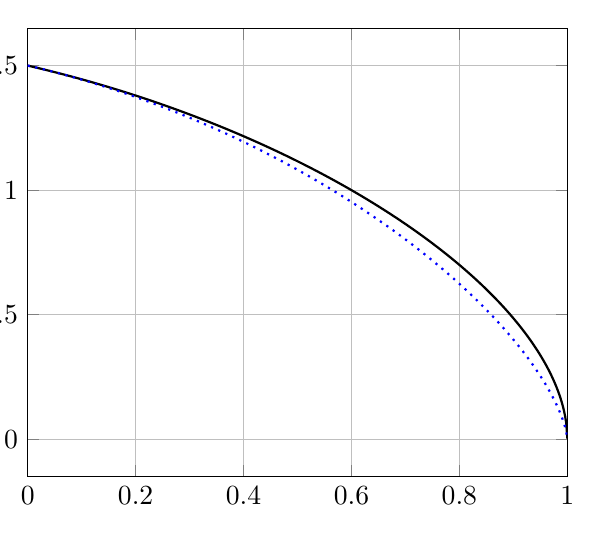
\begin{tikzpicture}[trim axis left,
    declare function={entropy(\x) = - \x * ln(\x)/ln(2) - (1 - \x) * ln(1 - \x) / ln(2); },
    declare function={gamma(\x) = (1 - x) / 2 + sqrt( 1 - x^2 ); },
    declare function={phi(\x) = (3/2) * (1 + x)^(1/3) * ( 1 - x )^(2/3); }
    %declare function = { entropy(\x) = 1; },
    ]
    \begin{axis}[domain=0:1,
      samples=500,
      enlarge x limits=false,
      grid=both,
      no markers]
      \addplot +[thick,black] { gamma(x) };
      \addplot +[thick,blue, dotted] { phi(x) };
    \end{axis}
  \end{tikzpicture}
  \qquad \qquad
  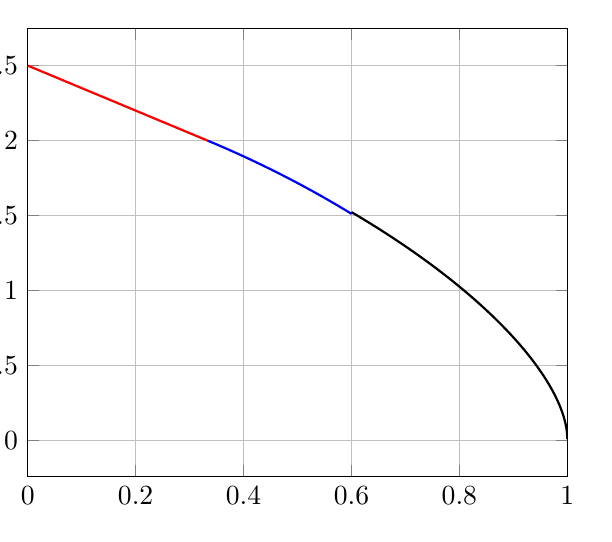
\begin{tikzpicture}[trim axis left,
    declare function={entropy(\x) = - \x * ln(\x)/ln(2) - (1 - \x) * ln(1 - \x) / ln(2); },
    declare function={gamma(\x) = (1 - x) / 2 + sqrt( 1 - x^2 ); },
    declare function={phi(\x) = (3/2) * (1 + x)^(1/3) * ( 1 - x )^(2/3); },
    declare function={psi(\x) = ( 1 - ln( (1+x)/(1-x) ) / ln(2) )^2 * ln(2) / 63; }
    %    declare function = { entropy(\x) = 1; },
    ]
    \begin{axis}[domain=0:1,
      samples=500,
      enlarge x limits=false,
      grid=both,
      no markers]
      \addplot +[thick,domain=0:(1/3),red] {(5 - 3 * x) / 2};
      \addplot +[thick,domain=(1/3):0.6,blue] {2^(2/3) * phi(x)};
      \addplot +[thick,domain=0.6:1,black] { 2^(2/3 + psi(x) ) * phi(x) )};
    \end{axis}
  \end{tikzpicture}
  
  \caption{\emph{(Left)} It is instructive to consider the base of the exponential part of the bounds on $\Exp[ g(W_{n-d+1}\cdots W_n) ]$. The solid curve is the $d$th root of the upper bound from Claim~\ref{claim:t2star-exact} and the dotted curve is the $d$th root of the lower bound from Claim~\ref{claim:t1star-exact}. We can see that beyond $\epsilon \geq 0.6$, the largest term in $\Exp[ g(W_{n-d+1}\cdots W_n) ]$ is $O(1)$. \emph{(Right)} We consider the same for $\Exp[ g(W_{n-d+1}\cdots W_n)^2 ]$. The curves depict the $d$th root of the upper bounds Claim~\ref{claim:t1star-variance-exact} and Claim~\ref{claim:t2star-variance-exact}. We can see that beyond $\epsilon \geq 0.81$, the largest term in $\Exp[ g(W_{n-d+1}\cdots W_n)^2 ]$ is $O(1)$.
  }
  \label{fig:grinding-power-mean}
\end{figure}

} % end iftoggle{drawfigs}

\iftoggle{drawfigs}{

\begin{figure}
  \centering
  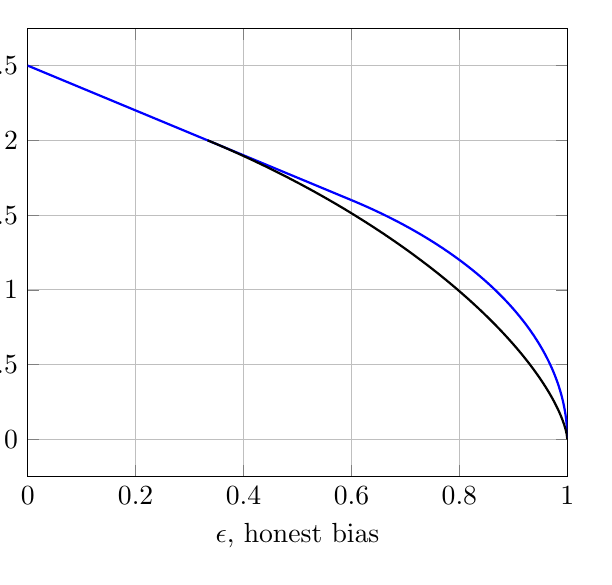
\begin{tikzpicture}[trim axis left,
    declare function={entropy(\x) = - \x * ln(\x)/ln(2) - (1 - \x) * ln(1 - \x) / ln(2); },
    %    declare function = { entropy(\x) = 1; },
    ]
    \begin{axis}[domain=0:1,
      samples=500,
      enlarge x limits=false,
      grid=both,
      xlabel={$\epsilon$, honest bias},
      no markers]
      \addplot +[thick,domain=0:(3/5),blue] {(5 - 3 * x)/2};
      \addplot +[thick,domain=(3/5):1,blue] {2 * sqrt( (1 - x^2))};
      % \addplot +[thick,domain=(3/5):1,red] {2 * sqrt( (1 - x^2))};
      \addplot +[thick,domain=(1/3):1,black] {(3/2^(1/3)) * (1+x)^(1/3) * (1-x)^(2/3)};
      % \addplot +[thick,domain=(3/5):1,black, dotted] {5/2 * (1 - x/2 - (6/25) * x^2 )};
      %\addplot +[thick,blue] { ((1-x)/2)^(2/3) * (1 + x)^(1/3) * 2^(entropy(x)) };

	  %\addplot +[thick,black] {(1-x)/2+sqrt(1 - x^2)};	
	  %\addplot +[thick,dotted,black] {(3/2)(1+x)^(1/3)(1-x)^(2/3)};	
    \end{axis}
  \end{tikzpicture}
  \caption{The blue curve is the $d$-th root of the bounds 
  from Proposition~\ref{prop:praos-moments-simple} and~\ref{prop:moments-t-large-eps}. 
  The black curve is the asymptotic bound from Claims~\ref{claim:t1star-variance-exact} and \ref{claim:t2star-variance-exact}.}
  \label{fig:grinding-power-variance}
\end{figure}

} % end iftoggle{drawfigs}


%=====================================================

\subsection{Proofs of the claims}
\subsubsection{Proof of Claim~\ref{claim:multiple-honest-blocks}}
    
  Let $m \in \NN$. 
  (Think of $m$ as the total number of honest participants. 
  However, as we show below, our analysis would not depend on $m$.)
  Consider the independent Bernoulli random variables $X_i \in \{0, 1\}, i \in [m]$ 
  and a tuple $(\sigma_1, \ldots, \sigma_m) \in [0,1]^m$ 
  so that $\Pr[X_i = 1] = \sigma_i$ 
  and $\sum \sigma_i = 1 - \alpha$. 
  Define $H_m = \sum_{i =1}^m X_i$ and observe that $\Exp H = 1 - \alpha$. 
  Then 
  $$
    A(\epsilon, \lambda) 
    = \Pr[W_1 \neq \A] \cdot \Exp[H^\lambda \mid H \geq 1]
    = (1-\alpha) \cdot \Exp[H^\lambda]/(1 - \Pr[H = 0])
    \leq \frac{1 - \alpha}{1 - e^{-(1 - \alpha)}} \cdot \Exp[H^\lambda]
  $$ 
  since $\Pr[H = 0] = \prod_i (1 - \sigma_i) \leq e^{-\sum_i \sigma_i} = e^{-(1 - \alpha)}$.
  Next, consider the i.i.d.\ Bernoulli random variables $X'_i \in \{0, 1\}, i \in [m]$ 
  so that $\Pr[X_i = 1] = (1-\alpha)/m$. 
  Define $H'_m = \sum_{i =1}^m X'_i$ and observe that $\Exp H = 1 - \alpha$. 

  % \begin{fact}\label{fact:mgf-equal-unequal-stake}
  %   For any integer $m \geq 1$ and positive real $\lambda$, 
  %   $\Exp e^{\lambda H'_m} \geq \Exp e^{\lambda H_m}$.
  % \end{fact}
  % \begin{proof}
  %   Writing $c = 1 - \alpha$, 
  %   the moment generating function of $H$ is 
  %   $$
  %     \Exp e^{\lambda H_m} 
  %     = \prod_i \Exp e^{\lambda X_i} 
  %     = \prod_i \left( (1 - \sigma_i)\cdot e^0 + \sigma_i \cdot e^\lambda  \right)
  %     = \prod_i \left(1 + \sigma_i(e^\lambda - 1) \right)
  %     = \prod_i (1 + \beta \sigma_i)
  %   $$
  %   where we write $\beta = e^\lambda - 1$. 
  %   By the AM-GM inequality, 
  %   the right-hand side above is at most 
  %   $$
  %     \prod_i (1 + \beta \sigma_i)
  %     \leq \left(\sum_{i=1}^m(1 + \beta \sigma_i)/m\right)^m 
  %     = (1 + \beta c/m)^m
  %     \,.
  %   $$
  %   On the other hand, 
  %   $$
  %     \Exp e^{\lambda H'_m} 
  %     = \prod_i \Exp e^{\lambda X'_i} 
  %     = \prod_i \left( (1 - c/m)\cdot e^0 + c/m \cdot e^\lambda  \right)
  %     = \prod_i (1 + \beta c/m)
  %     \geq \Exp H_m^\lambda
  %     \,.
  %   $$
  % \end{proof}



  Since the $X'_i$s are i.i.d., 
  \begin{align*}
    \Exp {H'_m}^2 
    &= \Exp \left(\sum_{i = 1}^m X'_i \right)^2
    = m \Exp {X'_1}^2 + \binom{m}{2} (\Exp X'_1)^2
    = m ((1-\alpha)/m) + \binom{m}{2} ((1 - \alpha)/m)^2 \\
    &= (1-\alpha) + \frac{m-1}{2m} (1 - \alpha)^2
    = (1-\alpha) \left( 1 + (1 - 1/m) (1 - \alpha)/2 \right) \\
    &\leq (1-\alpha) \left( 1 + (1 - \alpha)/2 \right)
    = (1-\alpha) (3 - \alpha)/2
    \,.    
  \end{align*}


  \begin{fact}\label{fact:second-moment-equal-unequal-stake}
    Let $m \in \NN$ and $c = \sum_{i = 1}^m \sigma_i$. 
    Then $\Exp H_m^2 \leq \Exp {H'_m}^2 \leq c + c^2$.
  \end{fact}
  \begin{proof}
    Writing $c = 1 - \alpha$, 
    \begin{align*}
      \Exp H_m^2 
      &=\Exp \left(\sum_i X_i\right)^2 
      = \sum_i \Exp X_i^2 + \sum_{i \neq j} (\Exp X_i)(\Exp X_j) 
      = \sum_i \sigma_i + \sum_i \sigma_i \sum_{j \neq i} \sigma_j 
      = c + \sum_i \sigma_i (c - \sigma_i) 
      = c + c^2 - \sum_i{\sigma_i^2}
      \,.      
    \end{align*}
    Similarly,
    \begin{align*}
      \Exp {H'_m}^2 
      &=\Exp \left(\sum_i X'_i\right)^2 
      = m \cdot c/m + m \cdot (c/m) (c - c/m) 
      = c + c^2 - c^2/m
      \,.      
    \end{align*}
    By the Cauchy-Schwartz inequality, 
    $
      c^2 = \left(\sum_i \sigma_i \right)^2 \leq m \, \sum_i \sigma_i^2
      % \,.
    $; the claim follows.
  \end{proof}

  It follows that 
  $$
    A(\epsilon, 2) 
    = \frac{1 - \alpha}{1 - e^{-(1 - \alpha)}} \cdot \Exp {H_m}^2
    \leq \frac{1 - \alpha}{1 - e^{-(1 - \alpha)}} \cdot \Exp {H'_m}^2
    \leq \frac{1 - \alpha}{1 - e^{-(1 - \alpha)}} \cdot (1-\alpha) (3 - \alpha)/2
    = \frac{(1 - \alpha)^2 (3 - \alpha)}{2 \left( 1 - e^{-(1 - \alpha)} \right)}
    \,.
  $$
  
  Since $\alpha = (1 - \epsilon)/2$, 
  we have 
  $1 - \alpha = (1 + \epsilon)/2$ 
  and 
  $3 - \alpha = (5 + \epsilon)/2$. 
  Therefore,
  $$
    A(\epsilon, 2) 
    \leq 
    % \frac{(1 - \alpha)^2 (3 - \alpha)}{2 \left( 1 - e^{-(1 - \alpha)} \right)}
    \frac{(1 + \epsilon)^2 (5 + \epsilon)}{16 \left( 1 - e^{-(1 + \epsilon)/2} \right)}
    \,.
  $$
  Finally, $\log_2 A(\epsilon, 2)$ is concave-increasing in $\epsilon \in (0, 1)$, 
  its linear approximation at $\epsilon = 0$ 
  is an upper bound to it. 
  Furthermore, we can check that this approximation is 
  bounded from above by the line $- 0.3 + 1.85 \epsilon$.
  \hfill$\qed$



\subsubsection{Proof of Claim~\ref{claim:t1star-variance-exact}}
  We use $\log$ to denote the base-$2$ logarithm and $H()$ to denote the binary entropy function. 
  Since $z \leq d/3$, $S(d,z)$ is at most $2^{d-z}$ and consequently, 
  $S(d, z)^2 B_{d, \epsilon}(d-z)$ is at most
  \begin{align}\label{eq:tz-variance-small-d}
  t_z&\defeq 2^{2(d-z)} \cdot (1-\epsilon)^d 2^{-d} {d \choose z}  \left(\frac{1+\epsilon}{1-\epsilon}\right)^{z} \nonumber \\
  &= 2^d(1-\epsilon)^d {d \choose z} \left(\frac{1+\epsilon}{4(1-\epsilon)}\right)^{z}\,.
  \end{align}
  Our goal is to bound $t_z$ from above. 

  % \paragraph{Case: $\epsilon < 1/3$.} 
  % Now we are dealing with the situation where $d \leq d/3$ and $\epsilon < 1/3$. 
  Let $\alpha \defeq z/d$ and observe that $\alpha \in [0, 1/3]$ since $z \leq d/3$.
  Using $z = \alpha d$ in~\eqref{eq:tz-variance-small-d} and 
  using the simplified bound $\binom{d}{\alpha d} \leq 2^{H(\alpha)d}$ from~\eqref{eq:nck}, 
  we can write
  \begin{align*}
  t_z
  &= 2^{d}(1-\epsilon)^d {d \choose \alpha d} \left(\frac{1+\epsilon}{4(1-\epsilon)}\right)^{\alpha d} \\
  &\leq 2^d
  (1-\epsilon)^d 
  2^{H(\alpha)d} 
  \left(\frac{1+\epsilon}{4(1-\epsilon)}\right)^{\alpha}
  \,.
  \end{align*}
  If we define 
  \begin{align*}
  q(\alpha, \epsilon)
  &\defeq H(\alpha)+1-2\alpha+ \alpha \log \frac{1+\epsilon}{1-\epsilon}+\log(1-\epsilon)
  \,,
  \end{align*}
  we can write $t_z = t_{\alpha d} \leq 2^{q(\alpha, \epsilon)d}$. 
  Thus our goal is to bound $q(\alpha, \epsilon)$ from above. 

  The function $q(\alpha, \epsilon)$ must be a unimodal concave function in $\alpha$ since for a fixed $\epsilon$, 
  it is a linear combination of $\alpha$ and the entropy function which is a unimodal concave function. 
  The largest term in the sequence $\{t_z\}$ corresponds to some $\alpha=\alpha^*$ that maximizes $q(\alpha, \epsilon)$. 
  % In order to bound $t_z$, it suffices to bound $q(\alpha^*, \epsilon)$. 
  The partial derivative of $q(\alpha, \epsilon)$ with respect to $\alpha$ is
  \begin{align*}
  \frac{\partial}{\partial \alpha}q(\alpha, \epsilon) &= -\log \frac{\alpha}{1-\alpha} - 2 + \log \frac{1+\epsilon}{1-\epsilon} 
  \,.
  % \frac{\partial^2}{\partial \alpha^2}q(\alpha, \epsilon) &= -\frac{1}{\alpha} - \frac{1}{1-\alpha} < 0
  % q^{(3)}(\alpha, \epsilon) &= \frac{1}{\alpha^2} - \frac{1}{(1-\alpha)^2} \\
  % q^{(4)}(\alpha, \epsilon) &= -\frac{2}{\alpha^3} - \frac{2}{(1-\alpha)^3} < 0
  \end{align*}
  The solution to the equation $\frac{\partial}{\partial \alpha}q(\alpha, \epsilon) = 0$ is given by
  % \begin{align*}
  % &\log (\frac{1}{\alpha} - 1) = 2 + \log\frac{1-\epsilon}{1
  % +\epsilon}\\
  % \text{or, }& \frac{1}{\alpha}-1 = \frac{4(1-\epsilon)}{1
  % +\epsilon} \\
  % \text{or, }&  \alpha^* \defeq \alpha^*(\epsilon) = \frac{1}{1+\frac{4}{r}} =  \frac{r}{4+r}\,,\\
  % \end{align*}
  $\alpha^* = r/(4 + r)$ where $r \defeq (1+\epsilon)/(1-\epsilon) < (1+1/3)/(1-1/3) = 2$.
  % Since $q(\alpha, \epsilon)$ is a linear combination of an $\alpha$-concave function (entropy) and linear terms in $\alpha$, $\alpha^*$ must maximize $q(\alpha, \epsilon)$. 

  We can substitute the definition of the binary entropy function $H(.)$ 
  in the definition of $q(\alpha, \epsilon)$ to get 
  \begin{align*}
  q(\alpha^*, \epsilon) 
  &= -\log\left[
  \left(\alpha^*\right)^{\alpha^*}(1-{\alpha^*})^{1-{\alpha^*}}
  \right] 
  + \log r^{\alpha^*} + 1 - 2{\alpha^*} + \log(1-\epsilon) \\
  &= -\log\left[ \left(\frac{r}{4+r}\right)^{\frac{r}{4+r}} \left(\frac{4}{4+r}\right)^{\frac{4}{4+r}}\right] 
   - \log \left(r^{-\frac{r}{4+r}} \right) + 1 - \frac{2r}{4+r}+\log(1-\epsilon) \\
  &= -\frac{1}{4+r} \log(4^4) + \log(4+r)+\frac{4-r}{4+r} + \log(1-\epsilon) \\
  &= \log\left[(4+r)(1-\epsilon)\right] - 1 \\
  &= \log\left[\left(4+\frac{1+\epsilon}{1-\epsilon}\right)(1-\epsilon)\right] - 1 \\
  &= \log(5-3\epsilon) - 1  = \log\left( (5 - 3 \epsilon)/2 \right)
  % \\
  % \implies 2^{q(\alpha, \epsilon)}
  % &\leq \frac{5-3 \epsilon}{2}
  \,.
  \end{align*} 
  Since $q(\alpha, \epsilon) \leq q(\alpha^*, \epsilon)$, we have 
  \[
      t_z \leq 2^{q(\alpha, \epsilon)d} \leq 2^{q(\alpha^*, \epsilon)d} = \frac{5 - 3 \epsilon}{2}
      \,.
  \]
  Although this bound holds for $\epsilon \in (0, 1)$, we claim this bound for only $\epsilon < 1/3$ 
  since we can in fact obtain a tighter bound for $\epsilon \geq 1/3$. 


  \paragraph{A tighter bound for $\epsilon \geq 1/3$.} 
  % First consider the case when $\epsilon \geq 1/3$. 
  We start by observing that $t_z$ increases monotonically in $z$ if $\epsilon \geq 1/3$. 
  To see this, note that the ratio of two consecutive terms in the sequence $t_0, t_1, t_2, \ldots$ is
  \[
  % r(z) \defeq
  \frac{t_{z+1}}{t_z} 
  =\frac{ {d \choose z+1} (1+\epsilon) }{ {d \choose z} 4(1-\epsilon) } 
  \geq \frac{(d-z)(1+\epsilon)}{4(z+1) (1-\epsilon)}\, .
  \]
  Since $\epsilon \geq 1/3$, this ratio is at least $(d-z)/2(z+1)$ which is 
  strictly greater than one for $z+1 \leq d/3$. 
  Hence the largest term in the sequence $\{t_z\}$ would be the last one. 
  Therefore,
  \begin{align*}
  t_z
  &\leq t_{d/3} = 2^d (1-\epsilon)^d 
  {d \choose d/3} 
  \left(\frac{1+\epsilon}{4(1-\epsilon)}\right)^{d/3} \\
  &\leq 2^{d/3}
  \frac{2^{H(1/3)d}}{\sqrt{ \pi (d/3) (2/3)}} 
  (1+\epsilon)^{d/3}(1-\epsilon)^{2d/3}  \qquad \text{using Corollary~\ref{coro:nchoosek_1}} \\
  &= \left( 2^{1/3 + H(1/3)} (1+\epsilon)^{1/3} (1-\epsilon)^{2/3} \right)^d \frac{3}{\sqrt{2 \pi d}} \\
  &= \left( 2^{2/3} \phi(\epsilon) \right)^d \frac{3}{\sqrt{2 \pi d}} 
  \qquad \text{using (\ref{eq:phi_eps}) and since }2^{1/3 + H(1/3)} = 3/2^{1/3}\\
  &\leq \left( 2^{2/3} \phi(\epsilon) \right)^d
  \end{align*}
  since $d \geq 2$. 

  It is not hard to check that 
  $2^{2/3} \phi(\epsilon)$ is at most $(5 - 3\epsilon)/2$ for $\epsilon \geq 1/3$. 
  First, check that they are equal at $\epsilon = 1/3$ and 
  at $\epsilon = 1$, $2^{2/3}\phi(1) = 0 < (5 - 3\cdot 1)/2 = 1$.
  Next, we establish the claimed
  inequality for respective logarithms. 
  In particular, let 
  \[
      a(\epsilon) = \ln\left( 2^{2/3} \phi(\epsilon) \right)
      \,,\qquad\text{and}\qquad 
      b(\epsilon) = \ln\left( (5 - 3 \epsilon)/2\right)
      \,.
  \]
  Check that the respective derivatives are 
  $a^\prime(\epsilon) = -(1+3 \epsilon)/3(1 - \epsilon^2)$ 
  and $b^\prime(\epsilon) = - 3/(5 - 3\epsilon)$. 
  Since both derivatives are negative, it remains to check that $|a^\prime(\epsilon)| \geq |b^\prime(\epsilon)|$. 
  To that end, we claim that the ratio $|a^\prime(\epsilon)|/|b^\prime(\epsilon)|$ 
  is strictly positive for $\epsilon > 1/3$. 
  To see this, observe that the ratio equals $(5 + 12 \epsilon - 9 \epsilon^2)/9(1-\epsilon^2)$. 
  For $\epsilon = 1/3 + \delta$ for any $\delta > 0$, 
  the numerator is $5 + 12 (1/3 + \delta) - 9 \epsilon^2$, 
  or $9(1 - \epsilon^2) + 12\delta$. 
  Since the denominator is $9(1 - \epsilon^2)$, the ratio is positive for $\epsilon \in(1/3, 1)$. 
\hfill$\qed$





\subsubsection{Proof of Claim~\ref{claim:t2star-variance-exact}}
  We use $\log$ to denote the base-$2$ logarithm and $H()$ to denote the binary entropy function. 
  Define $\alpha \defeq z/d \in (1/3, 1/2)$ and $r \defeq (1+\epsilon)/(1-\epsilon)$.
  Recall that $\binom{d}{\alpha d} \leq 2^{d H(\alpha)}$ using~\eqref{eq:nck}.
  Since $z$ is strictly larger than $(d - z)/2$, 
  we have the upper bound $S(d,z) \leq 2^{(d-z)H(z/(d-z))}$ from~\eqref{eq:S_d_z_large}). % S_d_z_upperbound

  % \begin{description}

  \paragraph{Case: $0 < \epsilon \leq 3/5$.} 
  % \item[Case: $0 < \epsilon \leq 3/5$.] 
  % In this case, $r = (1+\epsilon)/(1-\epsilon) \leq 4$.
  This gives
  \begin{align*}
  S(d, z)^2 B_{d,\epsilon}(d-z) 
  &\leq 2^{2(d-z)H(z/(d-z))} \cdot (1-\epsilon)^d 2^{-d} {d \choose z}  r^{z} \\
  % &\leq 2^{2(d-z)H(z/(d-z))} \cdot (1-\epsilon)^d 2^{-d} 2^{d H(z/d)}  \left(\frac{1+\epsilon}{1-\epsilon}\right)^{z} \\
  % &= \left( 2^{2(1-z/d)H(z/(d-z)) + H(z/d) - 1} \right)^d (1-\epsilon)^d 
  %  \left(\frac{1+\epsilon}{1-\epsilon}\right)^{z} \\
  &\leq \left( 2^{2(1-z/d)H(z/(d-z)) + H(z/d) - 1} \right)^d (1-\epsilon)^d r^{\alpha d} \\
   &= \left( 2^{ \alpha \log r + 2(1-\alpha)H(\alpha/(1 - \alpha)) + H(\alpha) - 1} (1-\epsilon) \right)^d 
  %  &= \left(2^{q(\alpha, \epsilon)} (1-\epsilon) \right)^d
  \,.
  \end{align*}
  % where we have used $4^z = 2^{2\alpha d}$. 
  Let us define 
  \[
      p(\alpha) \defeq 2 \alpha \log r + 2(1-\alpha)H(\alpha/(1 - \alpha)) + H(\alpha) - 1 
  \]
  so that 
  $
      S(d, z)^2 B_{d,\epsilon}(d-z) \leq \left(2^{p(\alpha)} (1-\epsilon) \right)^d
  $.

  Observe that $p(\alpha)$ is a unimodal concave function. 
  The derivative of this function is
  $
      -\left(4(1-2\alpha \log r)^4\right)/\left(\alpha^3(1-\alpha) \right)
  $
  which is strictly negative for $1/3 \leq \alpha < 1/2$. 
  It follows that $\alpha = 1/3$ (i.e., $z = d/3$) maximizes $p(\alpha)$. 
  Consequently,
  \begin{align*}
  S(d, z)^2 B_{d,\epsilon}(d-z)
  % &\leq S(d, d/3)^2 B_{d,\epsilon}(2d/3) \\
  &\leq \left(2^{q(1/3)} (1-\epsilon) \right)^d \\
  &= \left( 2^{(1/3)\log r + 2(2/3)H(1/2) + H(1/3) - 1}  (1-\epsilon) \right)^d \\
  &= \left( 2^{2(2/3)H(1/2) + H(1/3) - 1}  (1-\epsilon)
   \left(\frac{1+\epsilon}{1-\epsilon}\right)^{1/3} \right)^d \\
  &= \left( \frac{3}{2^{1/3}}  (1-\epsilon)
   \left(\frac{1+\epsilon}{1-\epsilon}\right)^{1/3} \right)^d \\
   &= \left(2^{2/3} \phi(\epsilon) \right)^d 
  \end{align*}
  since $2^{2^{1/3 + H(1/3)}} = 3/2^{1/3}$.

  \paragraph{Case: $3/5 < \epsilon \leq 0.81$.}
  % \item[Case: $3/5 < \epsilon \leq 0.81$.] 
  In this case, 
  \begin{align*}
  S(d,\alpha d)^2 B_{d,\epsilon}(d-\alpha d)
  &\leq \left( 2^{2(1-\alpha)H(\alpha/(1-\alpha)) + H(\alpha) - 1} \right)^d (1-\epsilon)^d 
   r^{\alpha d} \\
  &=\left( 2^{q(\alpha, \epsilon)} \right)^d\, ,
  \end{align*}
  where
  \begin{align*}
  q(\alpha, \epsilon)
  &\defeq H(\alpha) - 1 + 2(1-\alpha) H\left(\frac{\alpha}{1-\alpha}\right) 
  + \alpha \log r +\log(1-\epsilon)\,.
  \end{align*}
  Observe that $q(\alpha, \epsilon)$ is concave in $\alpha$ since for a fixed $\epsilon$, it is a linear combination of the concave entropy function and $\alpha$.  
  The derivatives of $q(\alpha, \epsilon)$ with respect to $\alpha$ are as follows:
  \begin{align*}
  d_1(\alpha) = \frac{\partial}{\partial \alpha}q(\alpha, \epsilon)
   &= \log \left(\frac{(1-2\alpha)^4}{\alpha^3(1-\alpha)}  \frac{1+\epsilon}{1-\epsilon} \right)\, .\\
  d_2(\alpha) = \frac{\partial^2}{\partial \alpha^2}q(\alpha, \epsilon)
  &= -\frac{3-2\alpha}{\alpha(1+2\alpha^2 -3\alpha) \ln 2} \\
  d_3(\alpha) = \frac{\partial^3}{\partial \alpha^3}q(\alpha, \epsilon)
  &= \frac{3-2\alpha( 3-2\alpha)^2}{\alpha^2(1+2\alpha^2 -3\alpha)^2 \ln 2}
  \, .
  \end{align*}
  We claim that $d_3(\alpha) < 0$ for $\alpha \in (1/3, 1/2)$. 
  To see this, let $f(\alpha) = 3 - 2\alpha(3 - 2\alpha)^2$. 
  Its derivative is $-2(3 - 2\alpha)(3 - 6\alpha)$ which is strictly negative for $\alpha \in (1/3, 1/2)$. 
  Hence $f(\alpha) < f(1/3) < 0$ and consequently, $d_3(\alpha) < 0$. 
  It follows that we can upper bound $q(\alpha, \epsilon)$ 
  by truncating its power series around $\alpha = 1/3$ 
  at the quadratic term. 
  The relevant derivatives at $\alpha = 1/3$ are 
  $d_1(1/3) = \log r - 1$ and
  $d_2(1/3) = -63/(2 \ln 2)$. 
  Thus $q(\alpha, \epsilon) \leq R(\alpha)$ where
  \begin{align*}
  R(\alpha)
  &= q(1/3, \epsilon) + (\alpha-1/3)\cdot d_1(1/3) + \frac{(\alpha-1/3)^2}{2}\cdot d_2(1/3) \\
  &= \left( H(1/3) - 1 + 4/3
      + (1/3)\log r + \log(1-\epsilon) \right)
      + (\alpha-1/3) \left( -1 + \log r \right)
      + \frac{(\alpha-1/3)^2}{2} \frac{-63}{2\ln 2}
  \\
  % &=  H(1/3) +2/3 - \alpha
  % + \alpha \log r + \log(1-\epsilon)
  % - (\alpha-1/3)^2 \cdot 63/(4\log_e 2) \\
  &= H(1/3) + 2/3 + \log(1-\epsilon) 
      + \alpha (\log r - 1) 
      - (\alpha-1/3)^2 \cdot 63/(4\ln 2)
      \,.
  \end{align*}
  % by ignoring the negative term.
  Its derivative is $R^\prime(\alpha)$ is $\log r - 1 - (\alpha - 1/3)63/(2 \ln 2)$. 
  The solution to the equation $R^\prime(\alpha) = 0$ is 
  $\alpha^* = 1/3 + \left( \log r - 1\right) (2 \log_e 2)/63$.
  This implies $q(\alpha, \epsilon) \leq R^*(\epsilon)$ for $\epsilon \in (0.6, 1]$ where
  \begin{align*}
      R^*(\epsilon)&\defeq R(\alpha^*) \\
      &= H(1/3) + 2/3 + \log(1-\epsilon)
          + \left( 1/3 + \left( \log r - 1\right) (2 \log_e 2)/63 \right) (\log r - 1) \\
      &{\quad}    - \left( (\log r - 1) (2 \ln 2)/63 \right)^2 \cdot 63/(4\ln 2) \\
      &= H(1/3) + 2/3 + \log(1-\epsilon)
          + (\log r - 1)/3 + (\log r - 1)^2 (2 \ln 2)/63  
          - (\log r - 1)^2 (\ln 2)/63 \\
      &= H(1/3) + 2/3 + \log(1-\epsilon)
          + (\log r - 1)/3 + (\log r - 1)^2 (\ln 2)/63  
          \,.
  % &= \log_2\left[ 
  %   \frac{3}{2^{1/3}} (1 + \epsilon)^{1/3} (1 - \epsilon)^{2/3} \right] 
  %   + \left(1 - \log_2 \frac{1+\epsilon}{1-\epsilon} \right)^2 \frac{ \log_e 2}{63} \\
  % &= \log_2\left[ 
  %   2^{2/3} \phi(\epsilon) \right] 
  %   + \left(1 - \log_2 \frac{1+\epsilon}{1-\epsilon} \right)^2 \frac{ \log_e 2}{63} \,.
  \end{align*}
  Since $2^{\log r - 1} = r/2$, we can compute
  \begin{align*}
      2^{R^*(\epsilon)}
      &= 2^{H(1/3)+2/3}(1-\epsilon) (r/2)^{1/3} (r/2)^{(\log r - 1)(\ln 2)/63} \\
      &= \phi(\epsilon) \cdot 2^{2/3} (r/2)^{(\log r - 1)(\ln 2)/63}
      \,,
  \end{align*}
  where we used~\eqref{eq:phi_eps} and the fact that $2^{H(1/3) + 2/3} = 3\cdot2^{-1/3}$.

  If $\epsilon \leq 0.81$, the factor $2^{2/3} (r/2)^{(\log r - 1)(\ln 2)/63}$ is at most $5/3$. 
  This gives us 
  \[
      S(d, z)^2 B_{d,\epsilon}(d-z) 
      \leq 2^{d q(\alpha, \epsilon)} 
      \leq 2^{R^*(\epsilon)} 
      \leq (5/3) \phi(\epsilon)
  \]
  for $\epsilon \in (3/5, 0.81]$.

  \paragraph{Case: $0.81 < \epsilon \leq 1$.}
  % \item[Case: $0.81 < \epsilon \leq 1$.]
  For the remainder of the proof, it suffices to establish
  \[
      q(\alpha, \epsilon) \leq q(\alpha, 0.81) \leq R^*(0.81) < 0
  \]
  for any $\epsilon \in (0.81, 1]$ and $\alpha \in (1/3, 1/2)$. 
  We already proved the inequality $q(\alpha, 0.81) \leq R^*(0.81)$ in the previous case. 
  A direct calculation shows that $R^*(0.81)$ is strictly negative; 
  hence $q(\alpha, 0.81)$ is strictly negative as well. 
  It remains to show that $q(\alpha, \epsilon) \leq q(\alpha, 0.81)$.
  We claim that the derivatives of $q(\alpha, \epsilon)$ and $R^*(\epsilon)$, 
  with respect to $\epsilon$, is negative for $\epsilon \in (0, 1]$ and $\alpha \in (1/3, 1/2)$. 
  Specifically,
  \begin{align*}
      \frac{d}{d\epsilon} q(\alpha, \epsilon)
      &= \alpha \dfrac{d}{d\epsilon} \left( \log(1+\epsilon) - \log(1-\epsilon)\right) 
          + \dfrac{d}{d\epsilon} \log(1-\epsilon) \\
      &= \frac{\alpha}{\ln 2}\left( 1/(1+\epsilon) + 1/(1-\epsilon)\right)
          - 1/(1-\epsilon) \\
      &= \frac{1}{(1-\epsilon)\ln 2}\left( \frac{2\alpha}{1+\epsilon} - 1\right) \\
      &\leq \left(\frac{1}{(1-\epsilon)\ln 2} \right) \cdot \left( \frac{1}{1+\epsilon} - 1\right) \\
      &< 0
  \end{align*}
  since the second factor above is negative while the first factor is positive.
  Hence $q(\alpha, \epsilon)$ is strictly negative for 
  $\epsilon \in [0.81, 1]$ and $\alpha \in (1/3, 1/2)$. 
  As a consequence,
  \[
      S(d, z)^2 B_{d,\epsilon}(d-z) 
      \leq 2^{d q(\alpha, \epsilon)} 
      \leq 1
      \,.
  \]

\hfill$\qed$